\section{\sysname 设计}
\label{sec:design}

\sysname 是一种基于 SGX 的高性能加密重复数据删除系统,专为外包存储而设计,尤其适用于具有高内容冗余的备份工作负载。 它旨在实现以下设计目标:(i){\em 机密性},即使在密钥服务器或任何客户端受到损害时,它也能保护外包块和密钥免受未经授权的访问,如 DupLESS \cite{bellare13b} 中的服务器辅助 MLE 和基于源的重复数据删除与 PoW \cite{halevi11}; (ii) {\em 带宽/存储效率},它在上传之前删除跨多个客户端的所有重复块,如基于源的重复数据删除。 (iii) {\em 计算效率},它减轻了加密操作的计算开销,并实现了比现有基于软件的加密重复数据删除设计更高的性能。

 
\subsection{概述}
\label{subsec:sgxdedup-arch}

图~\ref{fig:sgxdedup-overview}展示了\sysnameS 的系统框架,其分别在密钥服务器和每个客户端中引入了密钥安全区\textit{(Key Enclave)}和所有权证明安全区\textit{(PoW Enclave)}。

\begin{figure}[!htb]
    \centering
    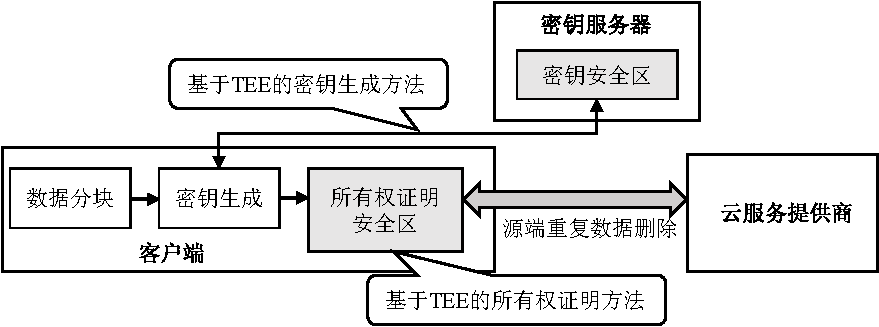
\includegraphics[width=\textwidth]{pic/sgxdedup/sgxdedup-arch.pdf}
    \caption{\sysnameS 系统框架,在密钥服务器和每个客户端中分别部署了密钥安全区和所有权证明安全区}
    \label{fig:sgxdedup-overview}
\end{figure}

\paragraph*{基于密钥安全区的服务器MLE密钥生成。}如图~\ref{fig:sgxdedup-overview-key}所示,\sysnameS 在密钥服务器中部署一个密钥安全区\textit{(Key Enclave)},以管理和保护服务器辅助消息锁加密所需的全局秘密$S$,使其免受恶意(例如,被攻击者攻击并取得控制权限)的密钥服务器的威胁。在执行服务器辅助消息锁加密密钥生成时,密钥安全区和客户端都首先基于共享的会话密钥(Blinded key)建立一个安全信道(有关如何生成会话密钥的详细设计,请参阅\S\ref{subsec:sgxdedup-key-management});然后客户端通过安全信道提交明文数据块的指纹;密钥安全区计算全局秘密和数据块指纹连接的结果的安全哈希作为该指纹对应的消息锁加密密钥;最后,密钥安全区通过安全信道向客户端返回该消息锁加密密钥。

\begin{figure}[!htb]
    \centering
    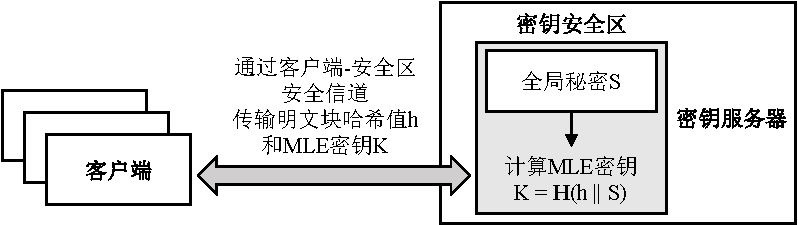
\includegraphics[width=0.9\textwidth]{pic/sgxdedup/key-enclave.pdf}
    \caption{基于密钥安全区的服务器辅助MLE密钥生成}
    \label{fig:sgxdedup-overview-key}
\end{figure}

密钥安全区同时实现了性能和安全性目标,它避免了在消息锁加密密钥生成期间使用昂贵的OPRF协议\cite{bellare2013DupLESS}。此外,它通过基于共享的会话密钥的安全信道保护数据块指纹和消息锁加密密钥,这样密钥服务器就无法从消息锁加密密钥生成过程中学习任何信息。此外,它可以有效保护安全区内存中的全局秘密$S$,即使密钥服务器受到攻击也能避免全局秘密的泄露,保障服务器辅助消息锁加密的安全性。但传统服务器辅助消息锁加密的安全性会由于全局秘密泄露而降低(\S\ref{subsec:background-encrypted-deduplication-key})。



\paragraph*{基于所有权证明安全区的数据块所有权证明。}如图~\ref{fig:sgxdedup-overview-pow}所示,\sysnameS 在每个客户端中部署一个所有权证明安全区,以证明源端重复数据删除中密文数据块的真实性。所有权证明安全区首先与云服务端协商生成一个共享的所有权证明密钥(\textit{PoW}密钥,本文目前使用Diffie-Hellman密钥交换(DHKE)实现密钥协商,参见\S\ref{sec:sgxdedup-implementation})。在生成消息锁加密密钥后,客户端将每个明文数据块加密为密文数据块。所有权证明安全区将密文数据块作为输入,计算相应的指纹,并使用与云服务端共享的PoW密钥创建该指纹的签名。随后,客户端将指纹和签名一起上传到云服务端。云服务端根据客户端对应的PoW密钥及指纹附加的签名验证指纹的真实性。只有当指纹被认证为真实有效时,云服务端才会继续检查指纹是否对应于任何已经存储的密文数据块副本。这里,本文验证客户端对密文数据块的所有权而不是明文的所有权(例如,\cite{halevi11}),以保护原始信息不被云服务端访问。由于消息锁加密产生的密文数据块与明文数据块一一对应,并且密文数据块的所有权与对应的明文数据块的所有权一致。因此,确保密文数据块的所有权足以保证安全。

\begin{figure}[!htb]
    \centering
    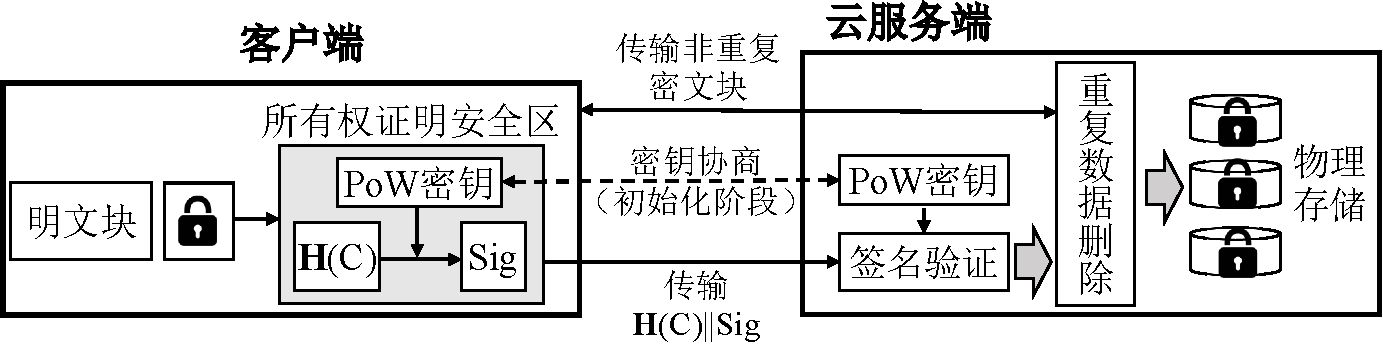
\includegraphics[width=\textwidth]{pic/sgxdedup/pow.pdf}
    \caption{\sysnameS 系统架构: 所有权证明安全区}
    \label{fig:sgxdedup-overview-pow}
\end{figure}


与密钥安全区相似,所有权证明安全区同样可实现效率与安全性的双重设计目标。它避免了基于密码学算法的所有权证明中Merkle树等结构的计算开销。同时,由于数据块是否已被云服务端存储的信息仅在数据块所有权验证通过后才会返回客户端,密钥安全区可有效保护重复数据删除系统免受恶意客户端的伪造数据所有权的攻击威胁。

\textbf{与现有研究\cite{kim2019ShieldStore,fuhry2020segshare,djoko2019NEXUS}在安全区内执行密钥生成和加密不同,本文选择在安全区之外执行数据块加密。}主要原因是原始明文数据块和加密过程都位于客户端内。被攻击的客户端本身可以直接访问其明文数据块,将加密过程移动到安全区内并不能提高安全性,同时还会导致安全区的计算开销增大、可信计算基大小增加。

\begin{table}[!htb]
    \small
    \centering
    \begin{tabular}{ccc}
        \toprule
        {\bf 所属安全区} & {\bf ECall名称}            & {\bf 描述}                                                           \\ 
        \midrule
        \multirow{5}{*}{\bf 密钥安全区}
                         & \textit{Secret generation} & 产生全局秘密 
        (\S\ref{subsec:sgxdedup-enclave-management})                                                                         \\
                         & \textit{Rekeying}          & 更新会话密钥 
        (\S\ref{subsec:sgxdedup-key-management})                                                                             \\
                         & \textit{Nonce checking}    & 检查nonce合规性 
        (\S\ref{subsec:sgxdedup-encryption})                                                                                 \\
                         & \textit{Key generation}    & 产生消息锁加密(MLE)密钥 (\S\ref{subsec:sgxdedup-encryption})         \\
                         & \textit{Mask generation}   & 生成加密掩码 (\S\ref{subsec:sgxdedup-encryption})                    \\
        \hline
        \multirow{3}{*}{\bf 所有权证明安全区}
                         & \textit{Key unsealing}     & 从磁盘解封所有权PoW密钥 (\S\ref{subsec:sgxdedup-enclave-management}) \\
                         & \textit{Key sealing}       & 密封所有权PoW密钥至磁盘 (\S\ref{subsec:sgxdedup-enclave-management}) \\
                         & \textit{Proof generation}  & 签名密文数据块对应的指纹 
        (\S\ref{sec:sgxdedup-implementation})                                                                                \\
        \bottomrule
    \end{tabular}
    \caption{\sysnameS 中的安全区内部调用(Ecalls)}
    \label{tab:sgxdedup-ecall}
\end{table}

\paragraph*{部署安全区存在的问题。}有效地实现基于TEE的加密后重复数据删除并非易事,因为本文需要减轻安全区的潜在性能开销,否则会抵消引入安全区带来的整体性能优势。本文提出了以下三个关键科学问题,并基于一套用于密钥安全区和所有权证明安全区(Table~\ref{tab:sgxdedup-ecall})的安全区内部调用来解决这些问题。

\begin{itemize}[leftmargin=0em]
    \item \textbf{如何安全有效地引导安全区?} (\S\ref{subsec:sgxdedup-enclave-management})由于密钥安全区需要维护全局秘密,在安全区启动时将全局秘密安全地载入密钥安全区中至关重要。此外,所有权证明安全区与客户端深度绑定,它应该在客户端在线访问云服务端时快速且安全的启动,并在客户端退出时以安全有效地方式终止。
    \item \textbf{密钥安全区和每个客户端应该如何建立安全信道?} (\S\ref{subsec:sgxdedup-key-management})
          每个客户端都基于共享的会话密钥与密钥安全区进行安全通信,以便生成必要的消息锁加密密钥来保护外包数据块。由于客户端可能随时加入或退出云存储服务订阅组,会话密钥不仅需要被高效协商产生,而且需要可以动态更新以进行动态客户端认证。
    \item \textbf{密钥安全区应该如何减少管理客户端安全信道的计算开销?} (\S\ref{subsec:sgxdedup-encryption})
          在每个安全信道中(密钥安全区和每个客户端之间),密钥安全区需要解密收到的数据块指纹并加密所生成的消息锁加密密钥。它的计算复杂度随着指纹数量和连接客户端的数量增加而增加。
\end{itemize}

\subsection{安全区管理}
\label{subsec:sgxdedup-enclave-management}

\sysnameS 在首次初始化时通过云建立对所有安全区的信任。在部署 \sysnameS 之前,本文首先将安全区代码编译成共享对象 \cite{sgx},为每个共享对象附加签名(用于完整性验证),并将共享对象分发到密钥服务器和每个客户端。云还托管共享对象以供后续验证。密钥服务器创建密钥安全区,而每个客户端通过加载相应的共享对象来创建自己的所有权证明安全区。云通过远程证明 (\S\ref{subsec:sgxdedup-sgx}) 对每个安全区进行身份验证,以确保加载正确的代码。在这里,本文解决了两个特定的管理问题:(i)如何将全局秘密(\S\ref{subsec:sgxdedup-arch})安全地引导到密钥安全区; (ii) 每个客户端在重启后如何有效地引导其所有权证明安全区。

\paragraph*{Key安全区management.} \sysnameS 不是完全引导全局密钥,而是根据云和密钥服务器分别拥有的两个 \textit{ sub-secrets} 在密钥安全区中生成全局密钥,以便阻止他们中的任何一个了解整个全球秘密。
为了生成全局密钥,本文将云的子密钥硬编码到密钥安全区代码中,并在 \sysnameS 初始化期间将代码(作为共享对象)传递给密钥服务器。本文还为密钥安全区实现了一个\textit{ secret generation ECall},以便让密钥服务器提供自己的子密钥。只有在云的子密钥被包含在密钥安全区中后,密钥服务器才能发出 ECall。它将密钥服务器的子密钥作为其单一输入,并对密钥服务器的子密钥和云的子密钥的串联进行哈希运算,形成全局密钥。请注意,密钥服务器无法访问安全区代码,因此无法了解在安全区内硬编码的云子秘密(假设逆向工程是不可能的)。因此,即使密钥服务器遭到破坏,全局秘密仍然是安全的,因此服务器辅助 消息锁加密(MLE) 的安全性得以保留。如果密钥服务器和云同时受到威胁,\sysnameS 的安全性会降低到原始 消息锁加密(MLE) (\S\ref{subsec:sgxdedup-encrypted-dedup}) 的安全性。

\paragraph*{所有权证明安全区管理。} 当客户端启动其 所有权证明安全区时,它​​需要证明 所有权证明安全区的真实性。但是,远程证明通常会产生非常大的延迟(例如,大约 9\,s;请参阅 \S\ref{subsec:sgxdedup-synthetic})以连接到Intel服务。与 key安全区不同,其远程证明只在初始化期间完成一次,客户端每次加入和离开 \sysnameS 时都需要分别引导和终止 PoW enclave。如果每次客户端加入时都使用远程证明,其大量开销将损害可用性。

\sysnameS 在 所有权证明安全区的第一次引导后利用密封来避免远程证明。回想一下,PoW 安全区与云共享一个PoW Key,这样云就可以验证指纹的真实性 (\S\ref{subsec:sgxdedup-arch})。本文的想法是根据 所有权证明安全区的测量哈希来密封PoW Key。因此,当客户端再次引导其所有权证明安全区时,它会将PoW Key解封到引导的所有权证明安全区中。只要成功恢复PoW Key,就可以验证自举 所有权证明安全区的真实性。

具体来说,客户端首先检查其物理机中是否有任何密封的PoW Key在本地可用。如果密封的PoW Key不可用(第一个引导程序),客户端通过远程证明来证明所有权证明安全区并与云交换PoW Key;否则,如果一个密封的PoW Key可用(在第一次引导之后),客户端通过加载共享对象创建一个新的 PoW enclave,并调用新 所有权证明安全区的 \textit{ key unsealing ECall} 来解封PoW Key。解封 ECall 的密钥以被密封的PoW Key的地址作为输入。它根据新 所有权证明安全区的测量散列推导出密封密钥,解密密封的PoW Key,并将其保存在新的 所有权证明安全区中。

当客户端离开 \sysnameS 时,它​​的 所有权证明安全区需要被终止。客户端发出 \textit{ key seal ECall} 来密封PoW Key。密钥密封 ECall 根据 所有权证明安全区的测量哈希对PoW Key进行加密,并将结果存储在客户端提供的地址中。
\subsection{可再生盲密钥管理}
\label{subsec:key-management}

每个客户端都通过一个共享的 \textit{ blinded} 密钥与密钥安全区安全通信,以防止密钥管理器 (\S\ref{subsec:arch}) 窃听。 为了形成盲密钥,一种直接的方法是直接在密钥安全区和每个客户端之间实现密钥协商协议。 但是,密钥安全区需要即时验证客户端(例如,客户端可以更新或撤销其云服务订阅)。 这种动态认证给密钥安全区带来了性能负担。


\begin{figure}[t]
\centering
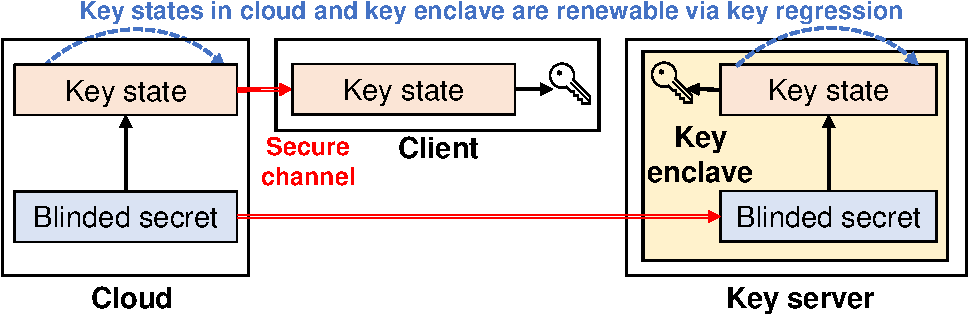
\includegraphics[width=\textwidth]{pic/sgxdedup/blindkey.pdf}
\vspace{-16pt}
\caption{可更新的盲密钥管理概述:云端和密钥安全区可以根据其盲密钥导出新的盲密钥,而客户端只能从云端下载一个密钥状态,并访问最新的盲密钥。}
\label{fig:keymanage}
\end{figure}

\sysname 在云的帮助下管理盲密钥。在初始化期间,云将一个不知情的秘密 $\kappa$ 硬编码到密钥安全区代码中。每个客户端从云端下载一个 \textit{ key state}(源自 $\kappa$;见下文),并生成其盲密钥(基于密钥状态)用于与密钥安全区的安全通信。我们的理由是双重的。首先,当客户端从云端发出任何下载请求时,云端可以检查客户端是否被授权。其次,我们可以从$\kappa$(而不是直接使用$\kappa$)派生一系列可更新的盲密钥,以防止被撤销/受损的客户端持续访问密钥安全区。作为附带的好处,可更新密钥管理还可以防止在线暴力攻击 (\S\ref{subsec:encrypted-dedup}),而不会主动降低密钥生成速率 \cite{bellare13b}。

\sysname 使用 \textit{ key regression} \cite{fu06} 导出可更新的盲密钥,同时确保每个客户端和密钥安全区中的盲密钥是一致的。具体来说,密钥回归适用于一系列密钥状态 $S[1]、S[2]、\ldots、S[m]$,每个状态都可用于派生密钥(例如,通过散列)。它允许密钥安全区和云执行 \textit{ rekeying} 以使用 \textit{ 密钥回归秘密从旧状态导出新状态(例如,从 $S[1]$ 导出 $S[2]$) },这样客户端就无法在不知道关键回归秘密的情况下了解有关新状态的任何信息。它还允许每个客户端从新状态派生任何旧状态(例如,从 $S[2]$ 派生 $S[1]$)。

为了在 \sysname 中实现密钥回归,我们使用 $\kappa$ 作为在云和密钥安全区之间共享的密钥回归秘密,用于派生新的状态和密钥。在每次上传时,客户端首先从云端下载最新的密钥状态$S[i]$,并请求密钥安全区接受的盲密钥的当前版本号$j$。鉴于密钥安全区可能无法及时更新盲密钥(例如,它正忙于在计划的更新密钥时间内准确地为密钥生成提供服务),$j$ 通常小于 $i$(即 $S[j]$在 $S[i]$) 之前。然后客户端从$S[i]$和对应的盲密钥$K[j]$推导出$S[j]$,并基于相同的$K[j]$与密钥安全区通信。请注意,云可以派生$K[j]$,但它不能窃听每个客户端和密钥安全区之间的通信,因为通过客户端和密钥管理器之间的基于 SSL/TLS 的通道额外保护了通信(参见我们在 \S\ref{subsec:threat} 中的假设)。

\sysname 更新云和密钥安全区中的盲密钥。 云实现了一个计时器,以在周期性的时间间隔内触发密钥更新。 密钥管理器发出 \textit{ rekeying ECall} 以在达到预定的密钥更新时间时触发密钥更新。

目前,我们实现了基于哈希的密钥回归方案 \cite{fu06} 以获得高密钥派生性能。 具体来说,我们定义了一个参数 $n$(现在设置为 $2^{20}$ \cite{fu06})来指示可承受的最大密钥更新次数。 云和密钥安全区计算第 i 个密钥状态为 $S[i] = {\bf H}^{n-i+1}(\kappa)$,每个客户端派生相应的盲密钥为 $K[i] = {\bf H}(S[i] || 0^8)$,其中${\bf H}^{n-i+1}()$迭代调用密码散列函数${ \bf H}()$ 乘以 $n-i+1$ 次,$||$ 是连接运算符。 为了导出旧状态,客户端下载 $S[i]$ 并恢复 $S[i-1] = {\bf H}(S[i])$。

\subsection{基于 SGX 的推测加密}
\label{subsec:encryption}

给定共享盲密钥 (\S\ref{subsec:key-management}),密钥安全区管理与每个客户端的安全通道,以在 MLE 密钥生成期间保护传输的指纹/密钥 (\S\ref{subsec:arch} )。然而,管理安全通道,特别是对于许多客户端,会在密钥安全区中产生高昂的加密/解密成本。 \sysname 在 SGX 的上下文中使用 {\em 推测加密} \cite{eduardo19} 增强了安全通信通道管理,从而减轻了密钥安全区的加密/解密开销。

\paragraph{推测加密} 推测加密 \cite{eduardo19} 采用{\em counter 模式} \cite{counter} 加解密,在离线过程中预先计算部分加解密结果,以减少在线独立加密文件系统中的计算开销。为了加密明文 $M$,我们首先将 $M$ 划分为一系列明文块 $b_1、b_2、\ldots、b_m$(例如,每个块的大小固定为 16 字节)。对于每个客户端,我们选择一个唯一的 {\em nonce} $\theta$,它只能被使用相同密钥的加密使用一次。然后我们计算第 $i$ 个明文块的 {\em 掩码}为 $e_i = {\bf E}(K, \theta || i)$,其中 ${\bf E}()$ 是对称加密函数,$K$ 是密钥,$i$ 是 {\em counter}(用于计数器模式加密),`$||$' 是连接运算符。最后,我们计算每个密文块$c_i = e_i \oplus b_i $,其中$\oplus$是按位异或运算符,并形成整个密文$C = c_1 || c_2 || \ldots || c_m$。为了解密密文,我们像上面一样为每个块生成掩码 $e_i$,恢复相应的明文块 $b_i = e_i \oplus c_i$ 并因此恢复原始明文 $M$。由于掩码生成步骤独立于每个目标明文/密文,我们可以离线预先计算掩码,然后应用轻量级 XOR 操作进行在线加密/解密。

\begin{figure}[t]
\centering
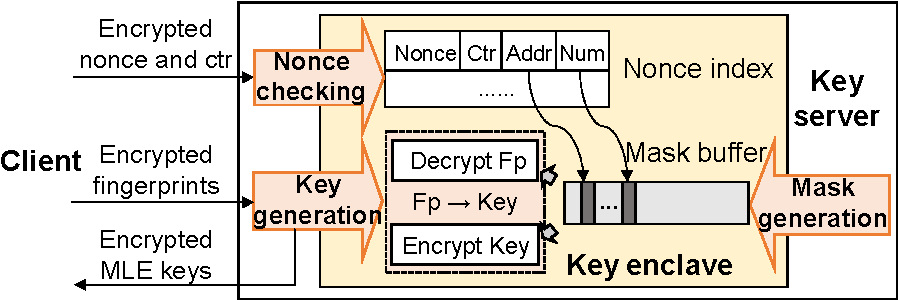
\includegraphics[width=3.3in]{pic/sgxdedup/encryption.pdf}
\caption{Overview of SGX-based speculative encryption.}
\label{fig:SpecEnc}
\end{figure}

\paragraph{Integration.} 要在 \sysname 中实现推测加密,我们需要解决 nonce、管理问题。、唯一的 nonce 充当不可预测的“一次性填充”,使得、每个 counter-mode 加密输出看起来随机 \cite{counter}。如果多个客户端使用反模式加密,我们需要在每个客户端的加密/解密操作中关联一个唯一的 nonce。但是,由于不同的客户端是隔离的,因此很难确保关联的 nonce客户是独一无二的。

为了确保 nonce 的唯一性,\sysname 在 key enclave 中管理一个集中的 key-value 存储,称为 {\em nonce index}。 nonce 索引的每个条目将存储的 nonce(12 字节)映射到三个字段:其计数器(4 字节)、相应掩码的起始地址(8 字节)和可用掩码的数量(4 字节)。此外,\sysname 实现了一个 {\em nonce checks ECall} (Figure~\ref{fig:SpecEnc}),它可以被密钥服务器调用,以将每个客户端提交的 nonce 与之前存储在 nonce 索引中的 nonce 进行比较,并如果发现重复的 nonce,通知客户重新选择一个新的。请注意,可以有效管理 in-enclave 随机数索引,因为它可以服务多达 112,000 个客户端(假设每个客户端一个随机数),只有 3MB EPC 空间(默认配置为 \sysname)。

\sysname 应用推测加密在客户端和密钥安全区之间建立安全通道,以保护 MLE 密钥生成。为了初始化安全通道,客户端将其自行选择的随机数 $\theta$ 和对应的计数器 $i$ 与密钥 enclave 同步,如果 $\theta$ 未用于任何加密,则 $i$ 初始化为零/由客户端解密。具体来说,它使用最新的盲密钥 (\S\ref{subsec:key-management}) 加密 $\theta$ 和 $i$,根据生成的密文计算消息验证码 (MAC),并将密文和 MAC 提交给密钥服务器。在这里,我们采用 {\em encrypt-then-MAC} \cite{bellare00} 通过检查 MAC 中的客户端和密钥安全区之间传输的任何信息来检测任何过时的盲密钥。

密钥服务器发出随机数检查 ECall,它将客户端的上传作为输入,解密 $\theta$ 和 $i$,并使用随机数索引检查解密后的 $\theta$ 和 $i$:
%
\begin{itemize}[leftmargin=*]
\item Case I:如果$\theta$ 是重复的并且$i$ = 0,这表示重复使用现有的nonce,并且ECall 返回一个信号通知客户端重新选择一个新的nonce。
\item 案例二:如果 $\theta$ 是重复的并且 $i \neq$ 为 0,这意味着 nonce 已被存储。 ECall 更新存储的计数器并标记相应的预计算掩码(用于后续处理,如下所述)。
\item 案例 III:如果 $\theta$ 是唯一的,这意味着 nonce 是新的,并且 ECall 将 $\theta$ 添加到 nonce 索引中。
\end{itemize}

对于 Cases~II 和 III,ECall 接受通信并要求客户端传输指纹以生成 MLE 密钥 (\S\ref{subsec:arch})。客户端根据$\theta$和$i$对指纹进行加密,并上​​传结果;在加密每个指纹块后,客户端将 $i$ 加一以防止重放攻击。如图~\ref{fig:SpecEnc}所示,密钥服务器发出{\em key generation ECall}来处理加密的指纹。 ECall 检查是否为当前客户端标记了某些掩码。如果找到(即情况 II),它使用标记的掩码来解密指纹并加密生成的 MLE 密钥。否则(即案例 III),它会在线计算掩码以进行解密和加密。

\paragraph{掩码预计算。} 为了加速加密/解密,当应用新的盲密钥(即所有现有掩码无效)或客户端在最后一个掩码后再次连接时,密钥安全区会执行掩码预计算代(即,它的一些掩码已被消耗)。关键安全区调用 {\em 掩码生成 ECall}(图~\ref{fig:SpecEnc}),它预先计算最近使用的随机数的数量(例如,在我们的例子中为三个)的掩码并写入将结果放入 {\em 掩码缓冲区}。默认情况下,我们将掩码缓冲区配置为最大 90\,MB。假设每个掩码占用 16 个字节,平均块大小为 8\,KB。指纹的 MLE 密钥生成使用四个掩码:两个用于解密 32 字节指纹,另外两个用于加密生成的 32 字节 MLE 密钥。因此,掩码缓冲区中预先计算的掩码可用于处理高达 11.25GB 数据的指纹。

